\documentclass[transparent]{beamer}
\usepackage[frenchb]{babel}
\usepackage[T1]{fontenc}
\usepackage[utf8]{inputenc}
\usepackage{ulem}
\usepackage{media9}
\usepackage{hyperref}
\usepackage{listings}
\usepackage{graphicx}
\usepackage{multicol}
\usetheme{Warsaw}
\useoutertheme{infolines}

\title{Drone paramoteur autonome}
\subtitle{PFEE}
\author{Benjamin  Ravalijaona - Nicolas DURAN - Rodolphe GUITTENY}
\institute{SCIA 2015 \\ EPITA}
\date{17 mai 2014}

\begin{document}

\begin{frame}
	\titlepage
\end{frame}

\begin{frame}
\begin{multicols}{2}
	\tableofcontents
\end{multicols}
\end{frame}

\section{Notre projet}
\AtBeginSection[]
  {
     \begin{frame}


     \frametitle{Plan}
\begin{multicols}{2}
     \tableofcontents[currentsection]
\end{multicols}
     \end{frame}
  }
\subsection{Présentation}

\begin{frame}

	\begin{block}{Le projet}
			\begin{itemize}
				\item Un drone paramoteur
				\item Equipé d'un téléphone 3G et d'une caméra GoPro
				\item Vol de manière autonome
				\item Détecte les voitures en excès de vitesse
				\item Intel Inside
			\end{itemize}
	\end{block}
\end{frame}

\subsection{Ojectifs}

\begin{frame}
	\begin{block}{Objectifs :}
			\begin{itemize}
				\item Détection de voitures en vol à partir d’image extraite de la GoPro fixée sur le drone.
				\item Estimation de la vitesse des voitures
				\item Detection d'une voiture roulant trop vite
				\item Suivi de la voiture par le drone (Tracking).
				\item Autonomie de l'appareil sur l'ensemble du trajet.
			\end{itemize}
	\end{block}
	\begin{block}{Remarque:}
			\begin{itemize}
				\item Le décollage et l’atterrissage du drone ne sont pas autonomes.
				\item Ces opérations seront télécomandé depuis une station de controle, manuellement.
			\end{itemize}
	\end{block}
\end{frame}

\section{Materiel}
\subsection{Le drone}

\begin{frame}
	\begin{block}{Le drone paramoteur Intel:}
			\begin{itemize}
				\item Fourni par Intel
				\item Armature en métal
				\item Moteur déjà fourni
				\item Hélice et batterie fourni
			\end{itemize}
	\end{block}
	\begin{block}{On ne le modifie pas}
			\begin{itemize}
				\item Hélice, moteurs et batterie déjà dimensionnés
				\item Précédents projets
				\item Charge utilse suffisante
			\end{itemize}
	\end{block}
\end{frame}

\begin{frame}
	\begin{block}{Un bon choix:}
			\begin{itemize}
				\item Autonomie
				\item Facilité de conduite
				\item Stabilité
				\item Sécurisant (il plane)
			\end{itemize}
	\end{block}
	\begin{block}{Mais :}
			\begin{itemize}
				\item Requiert de la place pour décoller/atterrir
				\item Pas de test en interieur possiible (comme avec un quadri-copter)
			\end{itemize}
	\end{block}
\end{frame}


\subsection{Telephone AZ210}

\begin{frame}
	\frametitle{Télehpone}
	\begin{center}
 	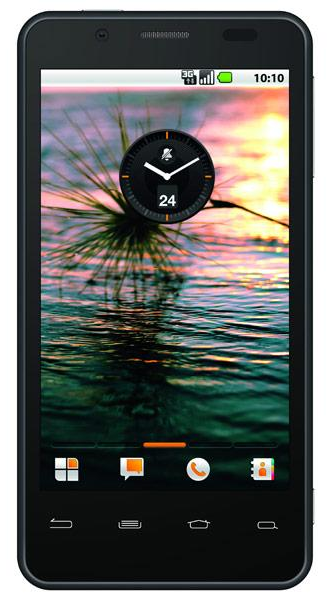
\includegraphics[height=0.8\textheight]{images/telephone.png} 
	\end{center}

\end{frame}

\begin{frame} 
	\begin{block}{Caractéristiques du téléphone:}
			\begin{itemize}
				\item RAM : 1Go
				\item CPU : Intel Atom Z2460 (1,6 Ghz)
				\item GPU : PowerVR SGX 540 overclocké à 400 MHz
				\item OS : Android 4.0.4 (ICS)
			\end{itemize}
	\end{block}
	\begin{block}{Choix du Téléphone:}
			\begin{itemize}
				\item Peu couteux proportionnellement au nombre de capteurs inclus.
				\item Facile d'utilisation
				\item Beaucoup de ressources (android)
				\item Fourni par Intel.
			\end{itemize}
	\end{block}
	\begin{block}{Mais :}
			\begin{itemize}
				\item Faible Puissance de calcul
			\end{itemize}
	\end{block}

\end{frame}

\subsection{GoPro HERO3 Silver Edition}
\begin{frame}
	\frametitle{Spécifications techniques générales}
	\framesubtitle{Telehpone}
	\begin{center}
 	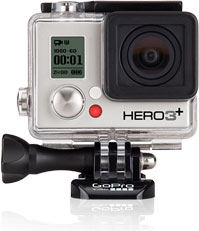
\includegraphics[height=0.8\textheight]{images/gopro.jpg} 
	\end{center}

\end{frame}

\begin{frame}
	\begin{block}{Caractéristiques de la GoPro:}
			\begin{itemize}
				\item Communication Wifi
				\item Image 10MP
				\item Rafales de 10 images/secondes
			\end{itemize}
	\end{block}
	\begin{block}{Ajout d'un appareil vidéo GoPro:}
			\begin{itemize}
				\item Bonne qualitée vidéo permettant des traitements de l'image.
				\item Possibilité de communicaton en wifi.
				\item Requiert un investissement.
				\item Utilisable par d'autre projet après nous
			\end{itemize}
	\end{block}
\end{frame}

\section{Communication}
\subsection{3G}

\begin{frame}
\frametitle{Un drone 3G-commandé}
	\begin{block}{Choix du réseau 3G:}
		\begin{itemize}
			\item Communication entre ordinateur et drone pour les controles manuels (décollage/atterrissage).
			\item Large couverture du réseau 3G
			\item Bascule en 2G si problème
			\item Capteur contenu dans le téléphone
			\item Norme internationale
		\end{itemize}
	\end{block}
	\begin{block}{Attention:}
		\begin{itemize}
			\item Latence acceptable mais variable
			\item Bande passante acceptable mais variable
		\end{itemize}
	\end{block}
\end{frame}

\subsection{WiFi}

\begin{frame}
\frametitle{Commande la GoPro par WiFi}
	\begin{block}{Choix du réseau Wifi:}
			\begin{itemize}
				\item Communication entre téléphone et appareil video GoPro.
				\item Bande passante importante.
				\item Faible latence.
			\end{itemize}
	\end{block}
	\begin{block}{Attention:}
			\begin{itemize}
				\item Consomme de la batterie
			\end{itemize}
	\end{block}
\end{frame}

\subsection{USB}

\begin{frame}
\frametitle{Commande la carte de controle par USB}
	\begin{block}{Contrôle de la carte commande:}
			\begin{itemize}
				\item Serial over USB
				\item Bibliothèque déjà existante
				\item Validé par le LSE
			\end{itemize}
	\end{block}
	\begin{block}{Attention:}
			\begin{itemize}
				\item Bibliothèque exempte de bug ?
			\end{itemize}
	\end{block}
\end{frame}
\addtocontents{toc}{\newpage}
\section{Nos outils informatique}
\subsection{Station de contrôle}

\begin{frame}
	\begin{center}
 	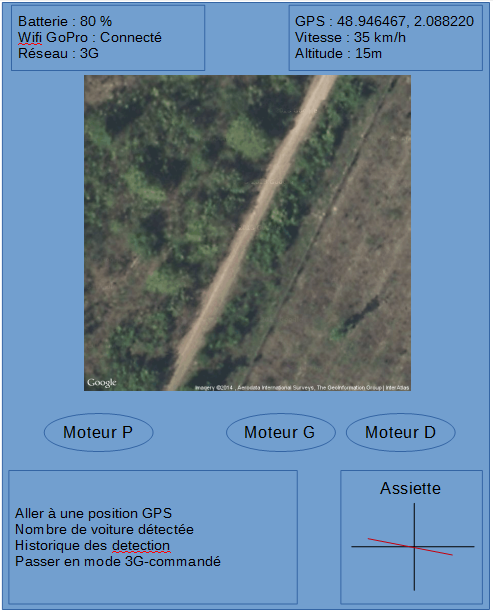
\includegraphics[height=0.95\textheight]{images/station.png} 
	\end{center}
\end{frame}

\begin{frame}
\frametitle{Une station de contrôle pour :}
	\begin{block}{Afficher :}
			\begin{itemize}
				\item Informations hardware (Batterie/Wifi)
				\item Informations de vol (vitesse, GPS, altitude)
				\item Assiette du drone
				\item Nombre de voitures détectées
			\end{itemize}
	\end{block}
	\begin{block}{Commander:}
			\begin{itemize}
				\item Aller à une position
				\item Arrêter de suivre une voiture
				\item Passer en mode autonome/3g-commandé
				\item Commander les moteurs
			\end{itemize}
	\end{block}
\end{frame}

\subsection{Environement de simulation}

\begin{frame}
	\frametitle{Un environement de simulation :}
	\begin{block}{Pour :}
			\begin{itemize}
				\item Tester nos algorithmes
				\item Ne pas casser de hardware
			\end{itemize}
	\end{block}
	\begin{block}{Fonctionnement}
			\begin{itemize}
				\item Basé sur la station de contrôle
				\item Remplacement des modules d'acquisitions
				\item Import d'un faux plan de vol de test (coordonées, images)
				\item Créations de tests
			\end{itemize}
	\end{block}
\end{frame}


\section{Tests}

\begin{frame}
\frametitle{Tests}
	\begin{block}{Images:}
			\begin{itemize}
				\item Utilisation de l'API Google Map en mode satellite
				\item Enregistrement d'images de tests dès le premier vol télécomandé
			\end{itemize}
	\end{block}
	\begin{block}{Plan de vol:}
			\begin{itemize}
				\item Rédigé manuellement
				\item Communauté des amateurs de drones
			\end{itemize}
	\end{block}
\end{frame}

\section{Analyse des risques}
\subsection{Risques}
\begin{frame}
\frametitle{Risques}
	\begin{block}{Risques:}
		\begin{itemize}
			\item Utilisation de code sous licenses non libres
			\item Légalisaté du vol de drone sur certaines zones (pas de permis de vol)
			\item Qualité non optimale de l'image lors de la capture d'image.
			\item Problème de précision lors de la direction du drone
			\item Possibilité de rencontre de perturbations et d'obstacles dans l'environnement durant le vol
			\item Puissance du téléphone insufisante
		\end{itemize}
	\end{block}
\end{frame}
\subsection{Solution}
\begin{frame}
\frametitle{Risques}
	\begin{block}{Solutions:}
		\begin{itemize}
			\item Utilisation de license libre
			\item Vol sur secteur restreint (champs)
			\item Gestion du rendu visuel par intermédiaire du GoPro
			\item Investissement principal sur l'environnement de simulation
			\item Algorithmes/Heuristiques optimisés, baisse de la qualité des images
		\end{itemize}
	\end{block}
\end{frame}

\section{Livrables}

\begin{frame}
\frametitle{Livrables}
	\begin{block}{Nos sources}
			\begin{itemize}
				\item La station de contrôle
				\item L'environement de simulation
				\item Le logiciel de contrôle du drone (Java)
				\item Une librairie de traitement d'image (C++)
			\end{itemize}
	\end{block}
	\begin{block}{Social}
			\begin{itemize}
				\item Un blog-photo retraçant tout le projet
				\item Une vidéo de présentation de nos résultats
			\end{itemize}
	\end{block}

\end{frame}

\section{Questions}

\begin{frame}[plain]
\begin{center}
\Huge Questions?
\end{center}
\end{frame} 

\end{document}
